\chapter{Trigonometry – Angles and Waves}

\section{Introduction: Understanding the World Through Trigonometry}
Trigonometry is the study of the relationships between the angles and sides of triangles, but it goes far beyond geometry. It has applications in fields like physics, engineering, architecture, and even sound and light waves. Whenever you hear terms like "sine" or "cosine," you're dealing with trigonometry.
In this chapter, we’ll explore the basics of trigonometry, focusing on how to understand angles, work with trigonometric functions, and apply these concepts to solve real-world problems involving triangles and waves.

\section{Right Triangles and Trigonometric Ratios}
The most common triangle in trigonometry is the right triangle, which has one angle equal to 90 degrees. The relationship between the sides and angles of a right triangle forms the foundation of trigonometry.
In any right triangle, we have three sides:
\begin{itemize}
    \item \textbf{Hypotenuse:} The longest side, opposite the right angle.
    \item \textbf{Opposite side:} The side opposite the angle you’re focusing on.
    \item \textbf{Adjacent side:} The side next to the angle you’re focusing on (but not the hypotenuse).
\end{itemize}

\begin{center}
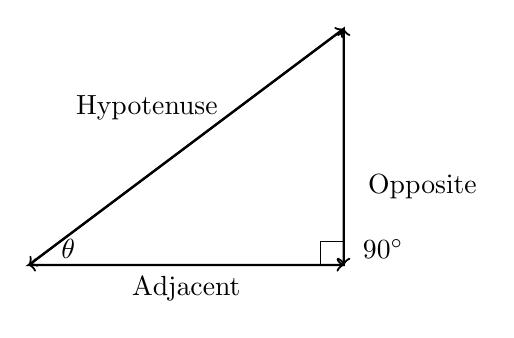
\begin{tikzpicture}
    % Draw the triangle
    \draw[thick] (0,0) -- (4,0) -- (4,3) -- cycle;

    % Labels for sides
    \node at (2, -0.3) {Adjacent};
    \node at (5,1) {Opposite};
    \node at (1.5, 2) {Hypotenuse};

    % 90 degree angle square
    \draw (3.7,0) rectangle +(0.3,0.3);
    \node at (4.5, 0.2) {$90^\circ$};

    % Angle label
    \node at (0.5, 0.2) {$\theta$};

    % Arrowed lines for sides
    \draw[thick, <->] (4,0) -- (4,3); % Opposite
    \draw[thick, <->] (0,0) -- (4,0); % Adjacent
    \draw[thick, <->] (0,0) -- (4,3); % Hypotenuse

\end{tikzpicture}
\end{center}

\subsection{Trigonometric Ratios}
The three basic trigonometric functions are sine (sin), cosine (cos), and tangent (tan). These functions relate the angles of a triangle to the lengths of its sides.
For any angle $\theta$ in a right triangle:
\begin{enumerate}
    \item \textbf{Sine (sin):}
    \[
    \sin(\theta) = \frac{\text{opposite}}{\text{hypotenuse}}
    \]
    \item \textbf{Cosine (cos):}
    \[
    \cos(\theta) = \frac{\text{adjacent}}{\text{hypotenuse}}
    \]
    \item \textbf{Tangent (tan):}
    \[
    \tan(\theta) = \frac{\text{opposite}}{\text{adjacent}}
    \]
\end{enumerate}
These ratios allow us to calculate missing side lengths or angles in right triangles.

\section{Using Trigonometric Ratios}
Let’s look at an example of how to use these trigonometric functions to solve problems involving right triangles.

\subsection{Example 1: Finding the Length of a Side}
In a right triangle, if the angle $\theta = 30^\circ$ and the hypotenuse is 10 units long, how long is the opposite side?
\begin{enumerate}
    \item Use the sine function:
    \[
    \sin(30^\circ) = \frac{\text{opposite}}{10}
    \]
    \item Look up or recall that $\sin(30^\circ) = 0.5$:
    \[
    0.5 = \frac{\text{opposite}}{10}
    \]
    \item Solve for the opposite side:
    \[
    \text{opposite} = 0.5 \times 10 = 5 \text{ units}
    \]
\end{enumerate}

\section{The Pythagorean Theorem}
The Pythagorean Theorem is another essential tool for working with right triangles. It relates the lengths of the sides of a right triangle:
\[
a^2 + b^2 = c^2
\]
Where:
\begin{itemize}
    \item $a$ and $b$ are the lengths of the legs (the two shorter sides),
    \item $c$ is the length of the hypotenuse.
\end{itemize}

\subsection{Example}
If one leg of a right triangle is 3 units long and the other leg is 4 units long, what is the length of the hypotenuse?
\begin{enumerate}
    \item Plug the values into the Pythagorean Theorem:
    \[
    3^2 + 4^2 = c^2
    \]
    \item Simplify:
    \[
    9 + 16 = c^2 \quad \Rightarrow \quad 25 = c^2
    \]
    \item Solve for $c$:
    \[
    c = \sqrt{25} = 5 \text{ units}
    \]
    The hypotenuse is 5 units long.
\end{enumerate}

\section{Angles in Degrees and Radians}
In trigonometry, angles can be measured in two different units:
\begin{enumerate}
    \item \textbf{Degrees:} The most familiar way to measure angles (e.g., $90^\circ$, $180^\circ$).
    \item \textbf{Radians:} A more mathematical way to measure angles, often used in calculus and advanced math. One full revolution around a circle is $2\pi$ radians, which is equivalent to $360^\circ$.
\end{enumerate}

\subsection{Converting Between Degrees and Radians}
To convert from degrees to radians, use the formula:
\[
\text{radians} = \frac{\pi}{180^\circ} \times \text{degrees}
\]

\subsubsection{Example}
Convert $90^\circ$ to radians:
\[
90^\circ = \frac{\pi}{180^\circ} \times 90^\circ = \frac{\pi}{2} \text{ radians}
\]

To convert from radians to degrees, use the formula:
\[
\text{degrees} = \frac{180^\circ}{\pi} \times \text{radians}
\]

\subsubsection{Example}
Convert $\frac{\pi}{4}$ radians to degrees:
\[
\frac{\pi}{4} \text{ radians} = \frac{180^\circ}{\pi} \times \frac{\pi}{4} = 45^\circ
\]

\section{The Unit Circle}
The unit circle is a circle with a radius of 1, centered at the origin of a coordinate plane. It’s a fundamental tool in trigonometry because it allows us to define the trigonometric functions for all angles, not just those in right triangles.
In the unit circle:
\begin{itemize}
    \item The x-coordinate of a point on the circle represents $\cos(\theta)$.
    \item The y-coordinate represents $\sin(\theta)$.
\end{itemize}

\subsection{Key Angles on the Unit Circle}
\begin{itemize}
    \item $\sin(0^\circ) = 0$ and $\cos(0^\circ) = 1$
    \item $\sin(90^\circ) = 1$ and $\cos(90^\circ) = 0$
    \item $\sin(180^\circ) = 0$ and $\cos(180^\circ) = -1$
    \item $\sin(270^\circ) = -1$ and $\cos(270^\circ) = 0$
\end{itemize}
Knowing these values allows you to solve trigonometric problems for many different angles.

\section{Graphs of Sine and Cosine}
The sine and cosine functions can be graphed as waves. These functions are periodic, meaning they repeat at regular intervals.

\subsection{Graph of Sine (sin)}
The sine wave starts at 0, rises to 1, falls back to 0, drops to -1, and returns to 0. This pattern repeats every $360^\circ$ or $2\pi$ radians.

\subsection{Graph of Cosine (cos)}
The cosine wave starts at 1, drops to 0, falls to -1, rises back to 0, and returns to 1. Like the sine wave, it repeats every $360^\circ$ or $2\pi$ radians.

\section{Applications of Trigonometry}
Trigonometry is incredibly useful in many real-world situations. Here are a few examples:
\begin{enumerate}
    \item \textbf{Engineering and Architecture:} Trigonometry helps engineers and architects design buildings, bridges, and other structures. They use trigonometric functions to calculate forces, angles, and distances.
    \item \textbf{Physics:} Trigonometry is used in physics to describe the motion of objects, especially those that move in waves, like sound and light. It’s also used to model oscillations, such as the swinging of a pendulum.
    \item \textbf{Navigation:} Trigonometry helps pilots and sailors navigate by using angles and distances on maps. It’s also crucial for understanding how GPS systems work.
    \item \textbf{Music and Sound Waves:} The sine and cosine functions describe sound waves. The pitch of a musical note is related to the frequency of the wave, which can be modeled using trigonometry.
\end{enumerate}

\section{Practice Makes Perfect: Let’s Try Some Exercises!}
\subsection{Trigonometric Ratios}
\begin{enumerate}
    \item Find $\sin(45^\circ)$ if the hypotenuse is 10 units.
    \item Find $\cos(30^\circ)$ if the hypotenuse is 8 units.
\end{enumerate}

\subsection{Right Triangles}
\begin{enumerate}
    \item Use the Pythagorean Theorem to find the missing side of a right triangle with legs of length 5 and 12.
    \item Find the tangent of an angle $\theta$ in a right triangle where the opposite side is 4 units and the adjacent side is 3 units.
\end{enumerate}

\subsection{Graphing}
\begin{enumerate}
    \item Sketch the graph of $y = \sin(x)$ for $0^\circ \leq x \leq 360^\circ$.
    \item Sketch the graph of $y = \cos(x)$ for $0^\circ \leq x \leq 360^\circ$.
\end{enumerate}

\section{Real-Life Applications of Trigonometry}
\begin{itemize}
    \item \textbf{Surveying:} Trigonometry is used in surveying to measure distances and angles between points on land.
    \item \textbf{Astronomy:} Astronomers use trigonometry to calculate the distances between stars and planets. The orbits of planets can be described using trigonometric functions.
    \item \textbf{Medical Imaging:} In technologies like MRI and ultrasound, trigonometry helps to create images of the inside of the human body by analyzing waves.
\end{itemize}

\section{Chapter Summary}
\begin{itemize}
    \item Sine (sin), cosine (cos), and tangent (tan) are the fundamental trigonometric ratios that describe the relationship between the sides and angles of a right triangle.
    \item The Pythagorean Theorem helps us find missing side lengths in right triangles.
    \item Angles can be measured in degrees or radians, and the unit circle is a key tool for understanding trigonometric functions for all angles.
    \item Sine and cosine functions can be graphed as periodic waves, repeating at regular intervals.
    \item Trigonometry has many practical applications, from engineering and architecture to physics, navigation, and music.
\end{itemize}

\section{Challenge Questions}

\begin{enumerate}

    % Question 1
    \item Find the height of a tree given the angle of elevation from a point 30 meters away is $45^\circ$.
    \begin{center}
        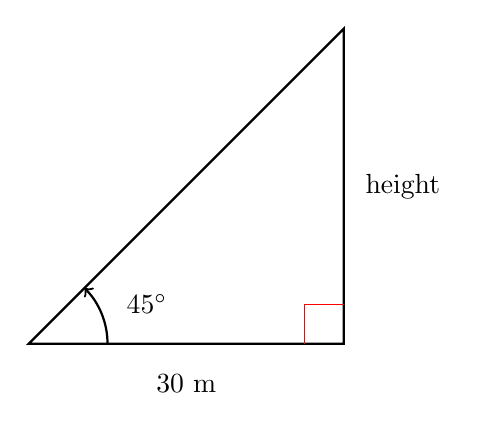
\begin{tikzpicture}
            \draw[thick] (0,0) -- (4,0) -- (4,4) -- cycle;
            \draw[red] (3.5,0) -- (3.5,0.5) -- (4,0.5);
            \node at (2, -0.5) {30 m};
            \node at (4.75, 2) {height};
            \draw[thick, ->] (1,0) arc[start angle=0, end angle=45, radius=1];
            \node at (1.5, 0.5) {$45^\circ$};
        \end{tikzpicture}
    \end{center}

    % Question 2
    \item A ladder leans against a wall at an angle of $60^\circ$ with the ground. If the ladder is 10 meters long, how far is the base of the ladder from the wall?
    \begin{center}
        \begin{tikzpicture}
            \draw[thick] (0,0) -- (6,0) -- (6,10) -- cycle;
            \draw[red] (5.5,0) -- (5.5,0.5) -- (6,0.5);
            \node at (2, 5) {10 m};
            \node at (3, -0.5) {Base distance};
            \draw[thick, ->] (1,0) arc[start angle=0, end angle=60, radius=1];
            \node at (1.5, 0.5) {$60^\circ$};
        \end{tikzpicture}
    \end{center}

    % Question 3
    \item Given a triangle with sides $a = 8$, $b = 15$, and an included angle $\theta = 60^\circ$, find the length of the third side.
    \begin{center}
        \begin{tikzpicture}
            \draw[thick] (0,0) -- (8,0) -- (4,6.92) -- cycle;
            \node at (4, -0.5) { a = 8};
            \node at (6.5, 4) {b = 15};
            \draw[thick, ->] (1,0) arc[start angle=0, end angle=60, radius=1];
            \node at (1.5,0.5) {$60^\circ \theta$};
        \end{tikzpicture}
    \end{center}

    % Question 4
    \item The sine of angle $\alpha$ in a right triangle is $\frac{3}{5}$. What is the cosine of the complementary angle $\beta$?
    \begin{center}
        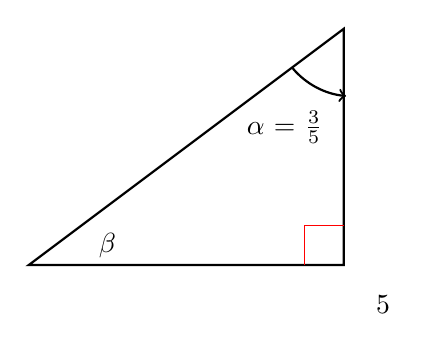
\begin{tikzpicture}
            \draw[thick] (0,0) -- (4,0) -- (4,3) -- cycle;
            \draw[red] (3.5,0) -- (3.5,0.5) -- (4,0.5);
            \node at (3.25, 1.75) {$\alpha$ = $\frac{3}{5}$};
            \draw[thick, ->] (3.35,2.5) arc[start angle=220, end angle=265, radius=1];
            \node at (1,0.25) {$\beta$};
            \node at (4.5, -0.5) {5};
        \end{tikzpicture}
    \end{center}

    % Question 5
    \item A point $P$ on the unit circle corresponds to an angle of $120^\circ$. Find the coordinates of point $P$.
    \begin{center}
        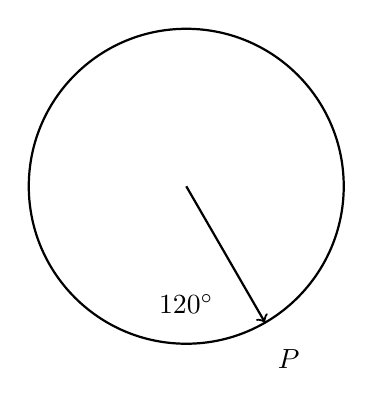
\begin{tikzpicture}
            \draw[thick] (0,0) circle (2);
            \draw[thick, ->] (0,0) -- (1,-1.73);
            \node at (1.3, -2.2) {$P$};
            \node at (0, -1.5) {$120^\circ$};
        \end{tikzpicture}
    \end{center}

    % Question 6
    \item Find the length of the shadow cast by a 5-meter pole when the sun's angle of elevation is $30^\circ$.
    \begin{center}
        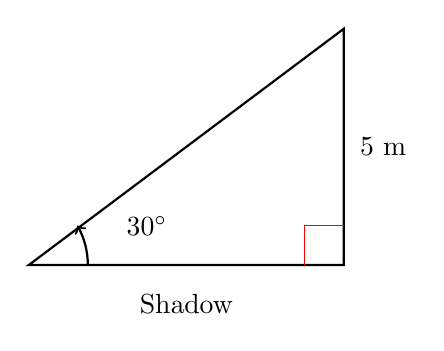
\begin{tikzpicture}
            \draw[thick] (0,0) -- (4,0) -- (4,3) -- cycle;
            \node at (4.5, 1.5) {5 m};
            \draw[red] (3.5,0) -- (3.5,0.5) -- (4,0.5);
            \node at (2, -0.5) {Shadow};
            \draw[thick, ->] (.75,0) arc[start angle=0, end angle=30, radius=1];
            \node at (1.5, 0.5) {$30^\circ$};
        \end{tikzpicture}
    \end{center}

    % Question 7
    \item Solve for $x$ in the equation $\tan(x) = \frac{1}{\sqrt{3}}$ for $0^\circ \leq x < 360^\circ$.
    \begin{center}
        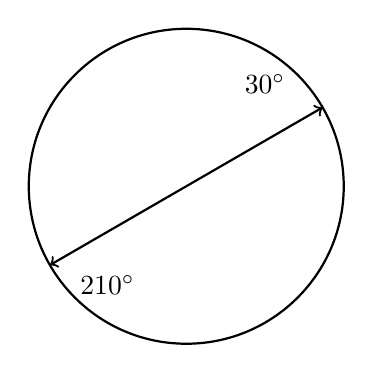
\begin{tikzpicture}
            \draw[thick] (0,0) circle (2);
            % Arrow for 30 degrees
            \draw[thick, ->] (0,0) -- (1.73, 1);
            \node at (1, 1.3) {$30^\circ$};
            % Arrow for 210 degrees
            \draw[thick, ->] (0,0) -- (-1.73, -1);
            \node at (-1, -1.25) {$210^\circ$};
        \end{tikzpicture}
    \end{center}

    % Question 8
    \item If $\sin(\theta) = 0.6$, find $\cos(\theta)$ using the Pythagorean identity.
    \begin{center}
        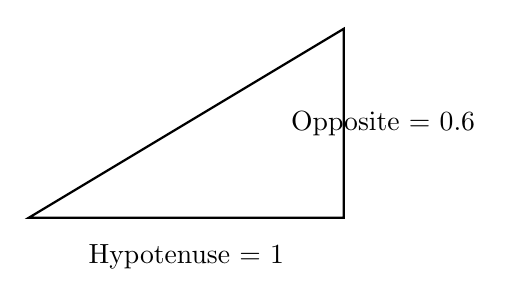
\begin{tikzpicture}
            \draw[thick] (0,0) -- (4,0) -- (4,2.4) -- cycle;
            \node at (4.5, 1.2) {Opposite = 0.6};
            \node at (2, -0.5) {Hypotenuse = 1};
        \end{tikzpicture}
    \end{center}

    % Question 9
    \item Find the area of a triangle with sides $a = 7$, $b = 9$, and angle $C = 45^\circ$ between them.
    \begin{center}
        \begin{tikzpicture}
            \draw[thick] (0,0) -- (7,0) -- (4,5) -- cycle;
            \node at (3.5, -0.5) {7};
            \node at (5, 2.5) {9};
            \node at (1, 3) {$45^\circ$};
        \end{tikzpicture}
    \end{center}

    % Question 10
    \item A ferris wheel has a radius of 20 meters. If a rider is at an angle of $\frac{\pi}{3}$ radians from the horizontal, what is their height above the ground if the wheel's center is 25 meters above the ground?
    \begin{center}
        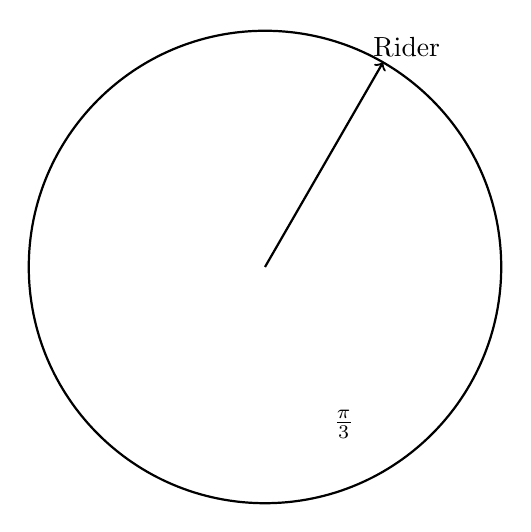
\begin{tikzpicture}
            \draw[thick] (0,0) circle (3);
            \draw[thick, ->] (0,0) -- (1.5,2.6);
            \node at (1.8, 2.8) {Rider};
            \node at (1, -2) {$\frac{\pi}{3}$};
        \end{tikzpicture}
    \end{center}

\end{enumerate}
